\documentclass[9pt,a4paper]{extarticle}
\usepackage[margin=13mm,headsep=4mm,footskip=7mm]{geometry}
\usepackage{amsmath,amssymb,booktabs,array,tabularx,multicol,graphicx,xcolor,enumitem,fancyhdr,hyperref}
\usepackage[most]{tcolorbox}
\definecolor{navy}{HTML}{17324D}\definecolor{blue}{HTML}{2D6A8A}\definecolor{pale}{HTML}{EEF5F8}\definecolor{warn}{HTML}{8A4B08}
\hypersetup{colorlinks=true,linkcolor=blue,urlcolor=blue}
\setlist{nosep,leftmargin=*}\setlength{\parindent}{0pt}\setlength{\parskip}{2.5pt}
\newcommand{\dd}{\,\mathrm{d}}
\newcommand{\unit}[1]{\,\mathrm{#1}}
\newcommand{\boxeq}[1]{\boxed{\displaystyle #1}}
\newtcolorbox{quick}[1][]{colback=pale,colframe=blue,boxrule=.5pt,arc=1mm,left=1.5mm,right=1.5mm,top=1mm,bottom=1mm,title=#1,fonttitle=\bfseries}
\newtcolorbox{trap}{colback=yellow!7,colframe=warn,boxrule=.5pt,arc=1mm,left=1.5mm,right=1.5mm,top=1mm,bottom=1mm,title=Common trap,fonttitle=\bfseries}
\pagestyle{fancy}\fancyhf{}\lhead{ENME601 Thermodynamics}\rhead{Half-Semester Open-Book Resource}\cfoot{\thepage}
\begin{document}
\begin{titlepage}
\centering\vspace*{25mm}
{\Huge\bfseries Thermodynamics\\Half-Semester Resource\par}\vspace{5mm}
{\Large ENME601 --- Weeks 1--6\par}\vspace{12mm}
{\large Compact open-book reference for systems, energy, properties, closed systems, control volumes and the second law\par}
\vfill
\begin{quick}[How to use this resource]
Start from the problem-type selector, write the complete mass/energy balance, then simplify only with stated assumptions. Use the separate tutorial booklet for source questions, official worked solutions and figures. Use the current \textit{Property Tables 2026} for numerical state properties.
\end{quick}
\vfill
{Compiled from the locally held 2026 course notes, current Weeks 1--6 tutorial sources, formula sheet and property tables.\\20 August 2026}
\end{titlepage}
\tableofcontents\newpage

\section{Exam-start decision system}
\begin{tabularx}{\textwidth}{>{\bfseries}p{.18\textwidth}X X}
\toprule
Problem cue & First model choice & Governing start point\\\midrule
Fixed mass, sealed tank, piston-cylinder & Closed system & $Q-W=\Delta U+\Delta KE+\Delta PE$\\
Inlets/outlets, nozzle, turbine, compressor, valve & Control volume & mass balance first; then SFEE\\
$P,T,x,v,u,h$ of water/refrigerant & Pure-substance state & classify phase, then select table\\
Gas far from saturation & Ideal gas & $PV=mRT$ plus appropriate energy relation\\
Liquid/solid heating & Incompressible & $\Delta u\simeq c\Delta T$; check pressure term in $\Delta h$\\
Engine/refrigerator/heat pump & Second law device & energy relation plus $\eta$ or COP\\\bottomrule
\end{tabularx}

\begin{quick}[Universal workflow]
\begin{enumerate}
\item Draw the boundary and label mass, heat and work arrows.
\item List knowns/unknowns; convert to absolute pressure and absolute temperature where required.
\item State assumptions (steady, adiabatic, rigid, ideal gas, negligible $\Delta KE/\Delta PE$, etc.).
\item Write unsimplified mass and energy balances before deleting terms.
\item Determine properties from the correct region/table; interpolate only after classification.
\item Substitute with units; check sign, magnitude and physical direction.
\end{enumerate}
\end{quick}

\section{Week 1 --- systems, state and basic properties}
\begin{multicols}{2}
\subsection{Definitions}
A \textbf{system} is the matter or region selected for study; the \textbf{surroundings} are everything else. The boundary may be fixed or moving.
\begin{center}\small
\begin{tabular}{lll}\toprule
Type & Mass crosses? & Energy crosses?\\\midrule
Closed/control mass & no & possibly\\
Open/control volume & yes & possibly\\
Isolated & no & no\\\bottomrule
\end{tabular}
\end{center}
Intensive properties do not scale with mass ($T,P,\rho,v$); extensive properties do ($m,V,U,E$). Specific properties divide an extensive property by mass.
\[
\rho=\frac{m}{V},\qquad v=\frac{V}{m}=\frac1\rho.
\]
A simple compressible state is fixed by \textbf{two independent intensive properties}. In a saturated mixture, $P$ and $T$ are dependent.

\subsection{Processes and cycles}
Isothermal: $T=$ const; isobaric: $P=$ const; isochoric: $V=$ const; adiabatic: $Q=0$. Heat and work depend on the path; properties depend only on end states. Over a cycle, every property has zero net change.

\subsection{Temperature and pressure}
\[
T[\mathrm K]=T[^{\circ}\mathrm C]+273.15,
\qquad P_{abs}=P_{atm}+P_{gauge},
\qquad P_{abs}=P_{atm}-P_{vac}.
\]
Use absolute $P$ and $T$ in gas and Carnot equations.

\begin{trap}
Steady does not mean uniform. Heat and work are boundary interactions, not properties stored in a system. Celsius temperature differences equal kelvin differences, but absolute-temperature ratios require kelvin.
\end{trap}
\end{multicols}

\section{Week 2 --- energy transfer, first law and ideal gases}
\begin{multicols}{2}
\subsection{Stored energy}
\[
E=U+KE+PE,
\quad e=u+\frac{V^2}{2}+gz,
\]
\[
\Delta KE=\frac{m(V_2^2-V_1^2)}2,
\qquad \Delta PE=mg(z_2-z_1).
\]
Velocity terms in SI are J/kg; divide by 1000 before adding to kJ/kg.

\subsection{Heat, work and sign convention}
This resource uses $Q>0$ into and $W>0$ by the system:
\[
\boxeq{Q-W=\Delta E}.
\]
For stationary closed systems, $Q-W=\Delta U$.
Heat is transfer caused solely by temperature difference. Work includes moving-boundary, shaft, electrical, spring, lifting and acceleration effects.
\[
\dot W_{shaft}=\tau\omega=2\pi N\tau,
\quad W_{spring}=\tfrac12k(x_2^2-x_1^2),
\quad W_{lift}=mg\Delta z.
\]

\subsection{Ideal-gas relations}
\[
\boxeq{Pv=RT},\qquad PV=mRT,\qquad R=\frac{R_u}{M}.
\]
For fixed mass:
\[
\frac{P_1V_1}{T_1}=\frac{P_2V_2}{T_2}.
\]
With $P$ in kPa and $V$ in m$^3$, $PV$ is kJ.

\begin{trap}
$Q=mc\Delta T$ is not the general first law. It is a property-change shortcut under a suitable model, with no phase change. Use $c_v$ for ideal-gas $\Delta u$ and $c_p$ for $\Delta h$.
\end{trap}
\end{multicols}

\section{Week 3 --- pure substances and property tables}
\subsection{Phase classification}
\begin{center}
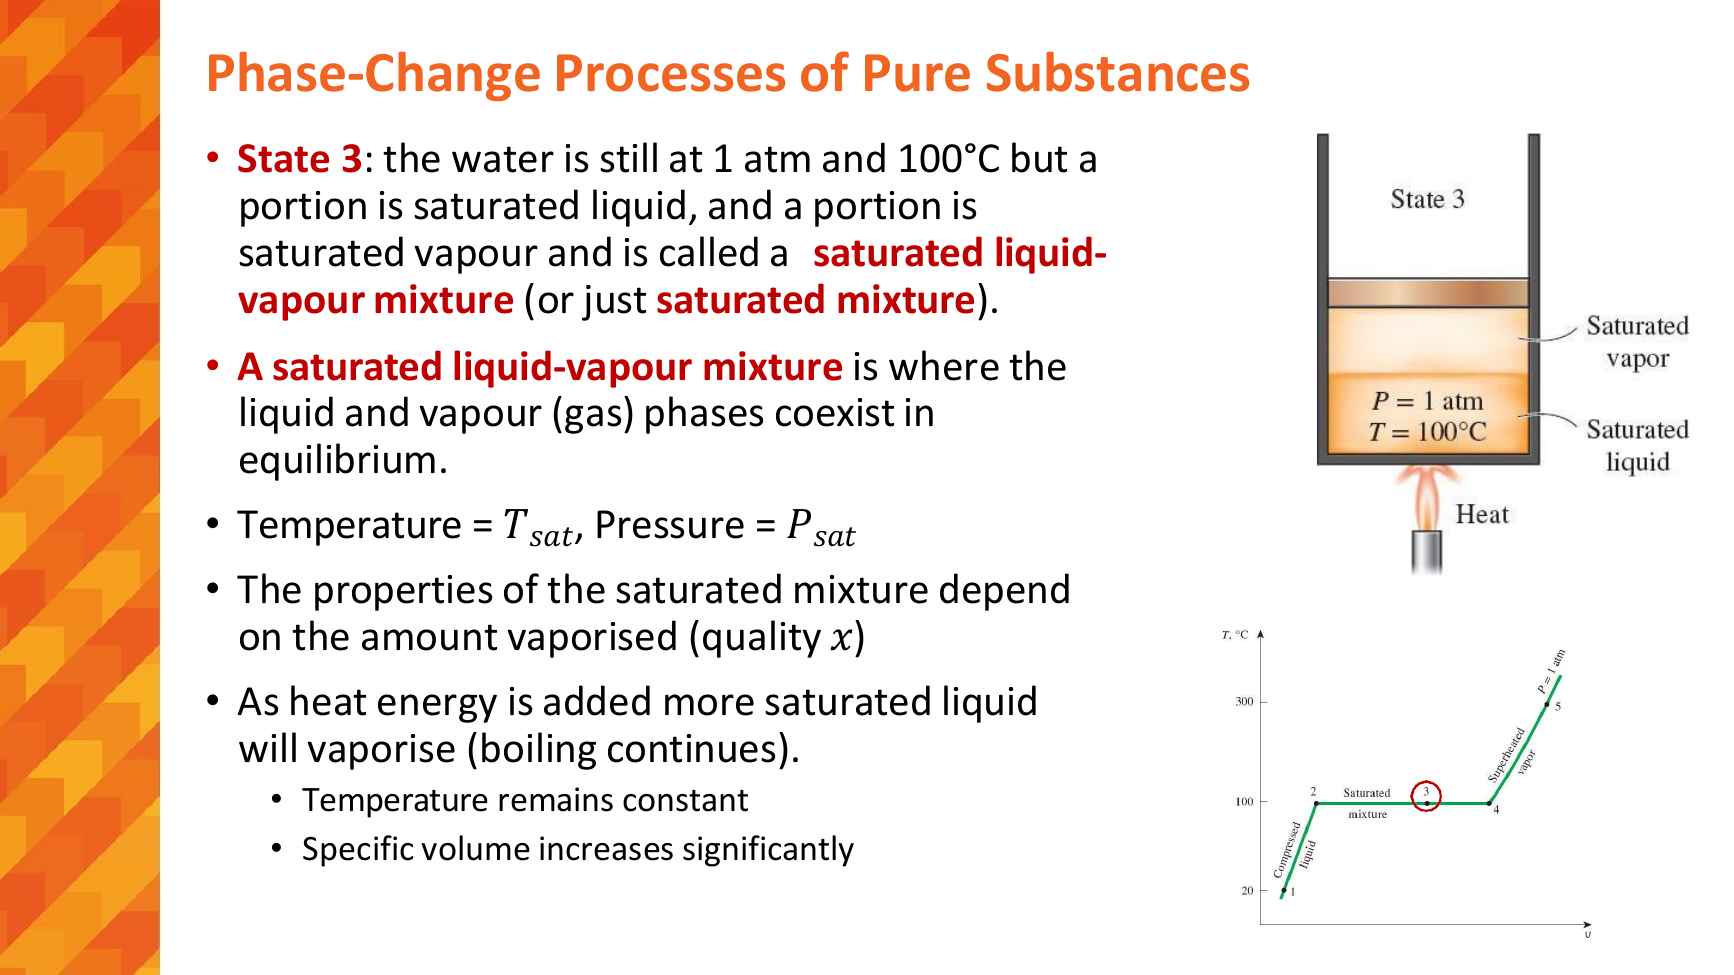
\includegraphics[width=.83\textwidth]{figures/week3-phase.png}
\end{center}
\begin{tabularx}{\textwidth}{>{\bfseries}p{.18\textwidth}p{.24\textwidth}X}
\toprule
Known at fixed $P$ & Region & Action\\\midrule
$T<T_{sat}(P)$ & compressed/subcooled liquid & compressed table or $y\approx y_f(T)$\\
$T=T_{sat}(P)$ & saturated state & another property or quality is required\\
$T>T_{sat}(P)$ & superheated vapour & superheated table\\\bottomrule
\end{tabularx}

\begin{multicols}{2}
\subsection{Saturation and quality}
Subscripts: $f$ saturated liquid, $g$ saturated vapour, $fg=g-f$.
\[
y_{fg}=y_g-y_f,
\qquad x=\frac{m_g}{m_f+m_g},
\]
\[
\boxeq{y=y_f+xy_{fg}},\qquad x=\frac{y-y_f}{y_{fg}},
\]
for $y\in\{v,u,h,s\}$. Quality is defined only inside the saturation dome and must satisfy $0\le x\le1$.

\subsection{Enthalpy and interpolation}
\[
h=u+Pv.
\]
Linear interpolation between entries $(X_1,y_1)$ and $(X_2,y_2)$:
\[
y=y_1+\frac{X-X_1}{X_2-X_1}(y_2-y_1).
\]
Never interpolate before selecting the correct region and table.

\subsection{Compressed-liquid approximation}
\[
y(T,P)\approx y_f(T),
\]
\[
h(T,P)\approx h_f(T)+v_f(T)[P-P_{sat}(T)].
\]

\begin{quick}[Fast table workflow]
Substance $\rightarrow$ two known intensive properties $\rightarrow$ compare with saturation $\rightarrow$ classify region $\rightarrow$ choose table $\rightarrow$ interpolate $\rightarrow$ sanity-check ordering. A mixture property must lie between its $f$ and $g$ limits.
\end{quick}
\end{multicols}

\section{Week 4 --- closed-system energy analysis}
\begin{center}
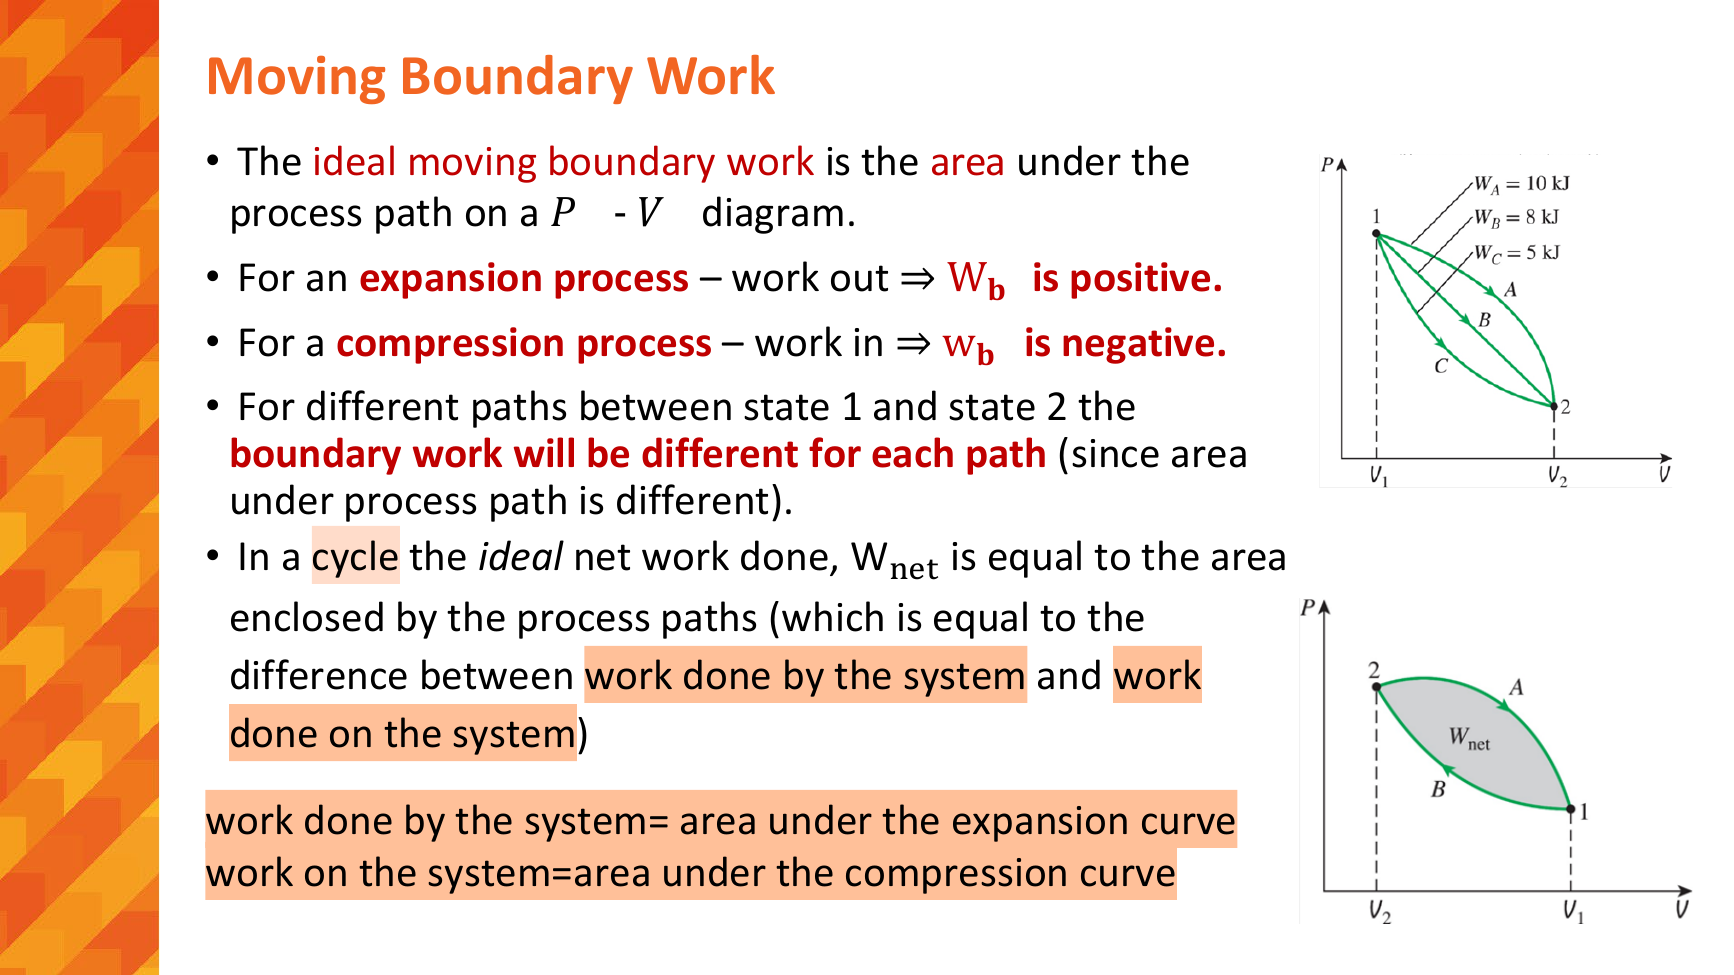
\includegraphics[width=.83\textwidth]{figures/week4-pv.png}
\end{center}
\begin{multicols}{2}
\subsection{Boundary work}
For quasi-equilibrium piston motion:
\[
\boxeq{W_b=\int_{V_1}^{V_2}P\dd V}.
\]
Expansion gives positive work by the system; compression gives negative work. Work is the area under the process path.

\begin{center}\small
\begin{tabular}{ll}\toprule
Model & Boundary work\\\midrule
Constant $P$ & $P(V_2-V_1)$\\
Rigid tank & $0$\\
Isothermal ideal gas & $mRT\ln(V_2/V_1)$\\
Polytropic, $n\ne1$ & $\dfrac{P_2V_2-P_1V_1}{1-n}$\\
Rev. adiabatic ideal gas & polytropic with $n=k$\\\bottomrule
\end{tabular}
\end{center}
For a polytropic process $PV^n=$ const. For a reversible adiabatic ideal-gas process $PV^k=$ const. Adiabatic alone is insufficient for the latter relation.

\subsection{Closed-system balance}
\[
Q-W=\Delta U+\Delta KE+\Delta PE.
\]
Stationary system: $Q-W=m(u_2-u_1)$. At constant pressure with boundary work as the only work:
\[
Q=\Delta H=m(h_2-h_1).
\]

\subsection{Specific heats}
\[
c_v=\left(\frac{\partial u}{\partial T}\right)_v,
\quad c_p=\left(\frac{\partial h}{\partial T}\right)_p.
\]
Ideal gas:
\[
\Delta u=\int c_v(T)\dd T\approx c_{v,avg}\Delta T,
\]
\[
\Delta h=\int c_p(T)\dd T\approx c_{p,avg}\Delta T,
\quad c_p-c_v=R,
\quad k=\frac{c_p}{c_v}.
\]
Incompressible liquid/solid:
\[
\Delta u\approx c\Delta T,
\qquad \Delta h\approx c\Delta T+v\Delta P.
\]

\begin{trap}
Constant pressure is not isothermal. Isothermal is not constant pressure. A rigid tank has $W_b=0$ but may still have heat, shaft or electrical work.
\end{trap}
\end{multicols}

\section{Week 5 --- control volumes and steady-flow devices}
\begin{center}
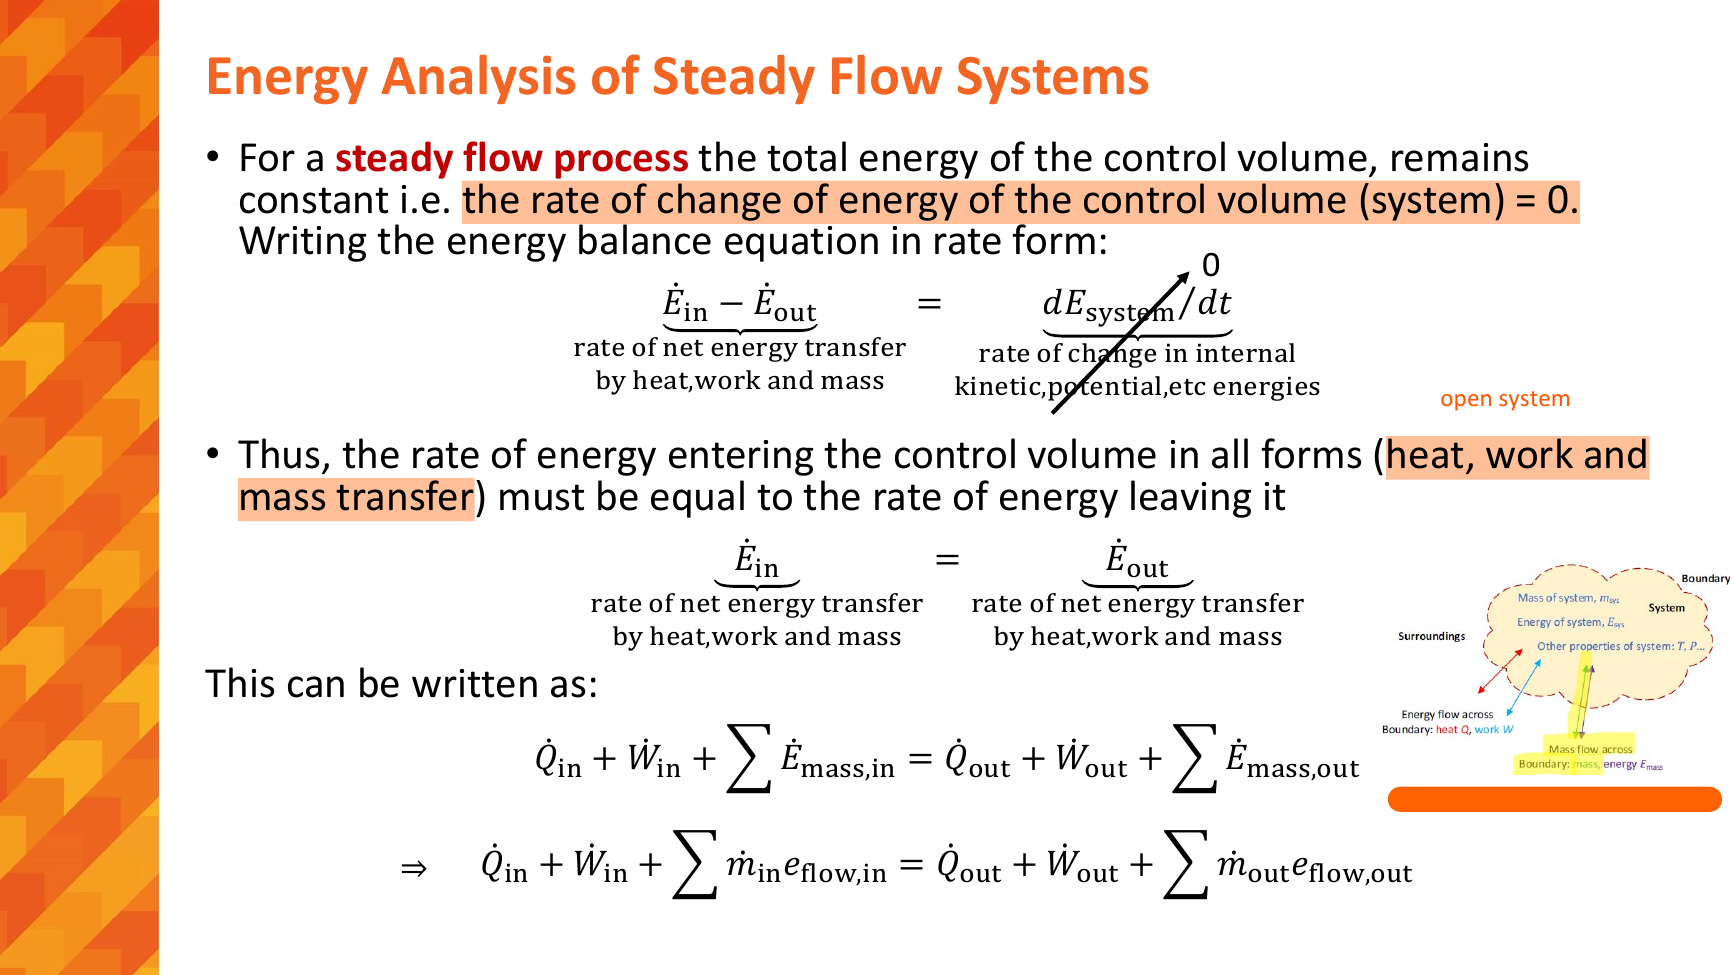
\includegraphics[width=.83\textwidth]{figures/week5-control-volume.png}
\end{center}
\subsection{Mass and stream energy}
\begin{multicols}{2}
\[
\dot V=V_{avg}A,
\qquad \boxeq{\dot m=\rho\dot V=\rho V_{avg}A=\frac{\dot V}{v}}.
\]
General mass balance:
\[
\sum\dot m_{in}-\sum\dot m_{out}=\frac{dm_{CV}}{dt}.
\]
At steady state, $\sum\dot m_{in}=\sum\dot m_{out}$. Flow work $Pv$ combines with $u$ to form enthalpy, so a stream carries
\[
e_{flow}=h+\frac{V^2}{2}+gz.
\]

\subsection{Steady-flow energy equation}
Using heat in and work out as positive:
\[
\dot Q-\dot W=\sum_{out}\dot m\left(h+\frac{V^2}{2}+gz\right)-\sum_{in}\dot m\left(h+\frac{V^2}{2}+gz\right).
\]
One inlet and outlet:
\[
\boxeq{\dot Q-\dot W=\dot m\left[\Delta h+\frac{V_2^2-V_1^2}{2}+g(z_2-z_1)\right]}.
\]
Write mass balance first. Simplify only after inspecting the device.
\end{multicols}

\subsection{Device selector}
\begin{tabularx}{\textwidth}{>{\bfseries}p{.18\textwidth}X X}
\toprule
Device & Typical assumptions & Dominant result\\\midrule
Nozzle/diffuser & steady, adiabatic, no shaft work, $\Delta PE\simeq0$ & $h_1+V_1^2/2=h_2+V_2^2/2$\\
Turbine & adiabatic, $\Delta KE,\Delta PE\simeq0$ & $\dot W_{out}=\dot m(h_1-h_2)$\\
Compressor & adiabatic, $\Delta KE,\Delta PE\simeq0$ & $\dot W_{in}=\dot m(h_2-h_1)$\\
Pump, incompressible & small $\Delta T$ & $w_{in}\simeq v(P_2-P_1)$\\
Throttle & adiabatic, no work, negligible $\Delta KE,\Delta PE$ & $h_1=h_2$\\
Mixing chamber & adiabatic, no work & mass balance plus $\sum\dot m h_{in}=\sum\dot m h_{out}$\\
Heat exchanger, whole & externally adiabatic, no work & hot-stream loss = cold-stream gain\\
Filling/emptying tank & transient, not steady & integrated mass and uniform-flow energy balances\\\bottomrule
\end{tabularx}

\begin{trap}
A constant inlet flow does not make a filling tank steady: mass accumulates. Throttling is isenthalpic, not necessarily isothermal or isentropic. Distinguish speed $V$ from volume flow rate $\dot V$.
\end{trap}

\section{Week 6 --- second law, engines, refrigeration and Carnot limits}
\begin{center}
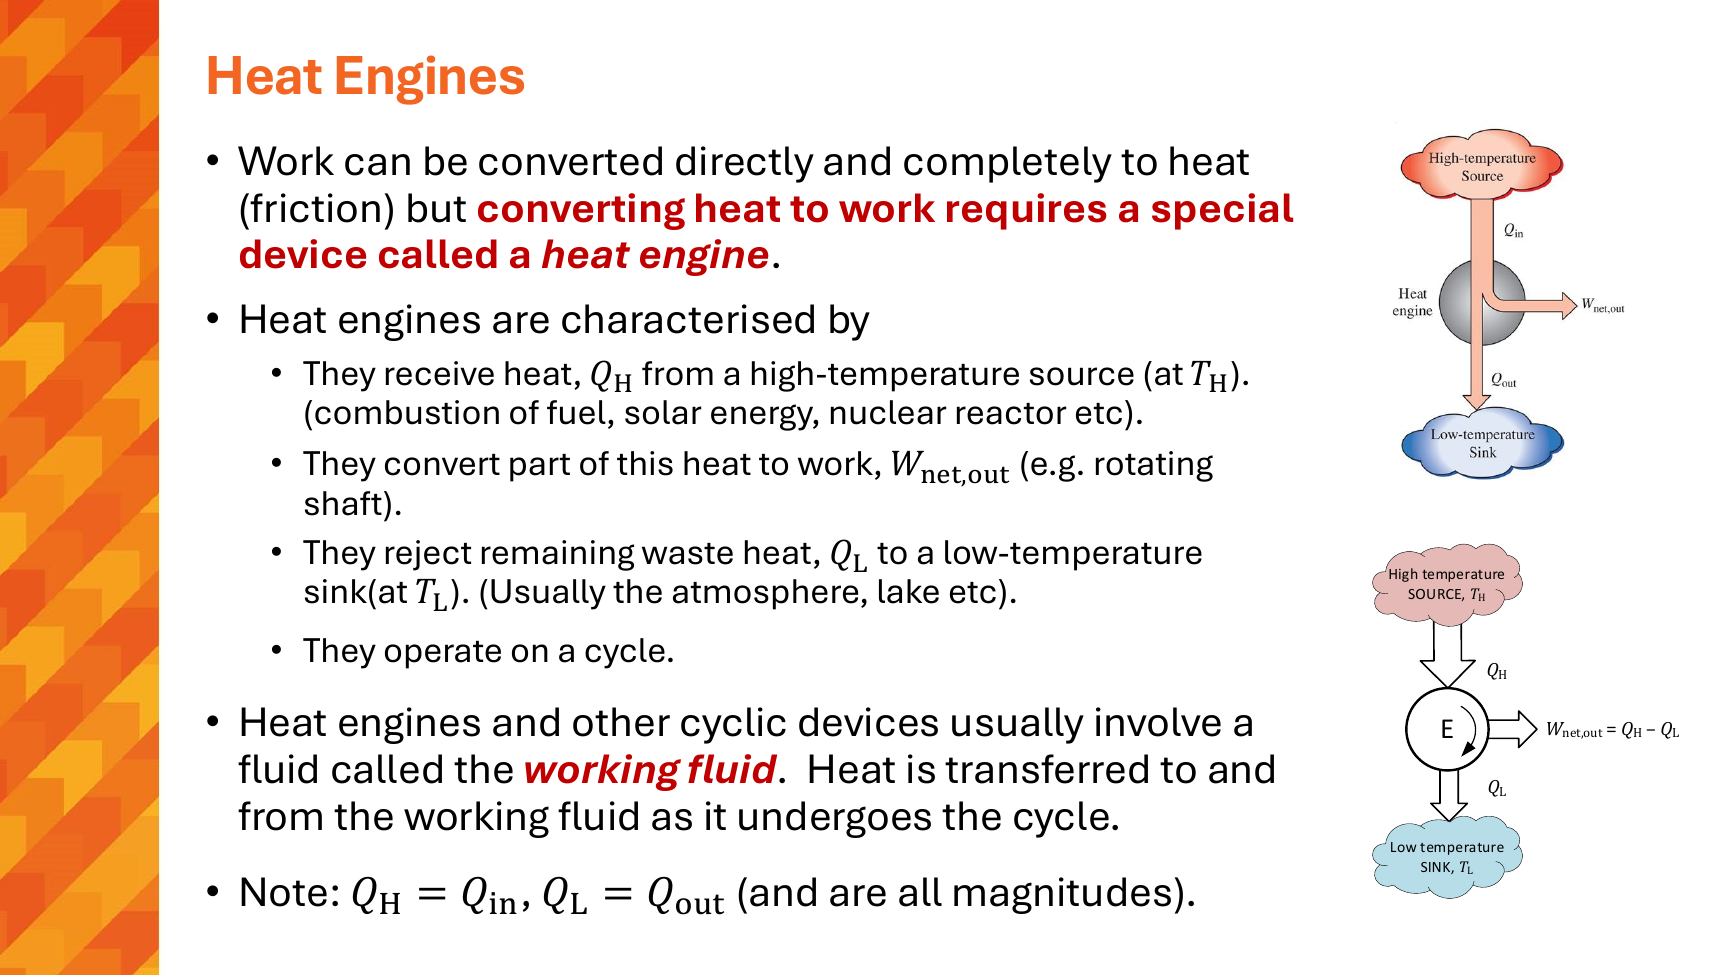
\includegraphics[width=.83\textwidth]{figures/week6-engine.png}
\end{center}
\begin{multicols}{2}
\subsection{Heat engine}
\[
W_{net,out}=Q_H-Q_L,
\quad \boxeq{\eta_{th}=\frac{W_{net,out}}{Q_H}=1-\frac{Q_L}{Q_H}}.
\]
A cyclic engine must reject heat; a 100\% heat engine violates Kelvin--Planck.

\subsection{Refrigerator and heat pump}
\[
W_{net,in}=Q_H-Q_L,
\]
\[
\boxeq{COP_R=\frac{Q_L}{W_{net,in}}},
\qquad \boxeq{COP_{HP}=\frac{Q_H}{W_{net,in}}=COP_R+1}.
\]
A COP above one is normal because work moves additional heat; COP is not heat-engine efficiency.

\subsection{Carnot limits}
For reservoirs at absolute temperatures $T_H$ and $T_L$:
\[
\boxeq{\eta_{th,rev}=1-\frac{T_L}{T_H}},
\]
\[
\boxeq{COP_{R,rev}=\frac{T_L}{T_H-T_L}},
\qquad \boxeq{COP_{HP,rev}=\frac{T_H}{T_H-T_L}}.
\]
A real device cannot exceed the reversible limit for the same reservoirs.

\subsection{Reversibility}
Irreversibilities include friction, unrestrained expansion, mixing, heat transfer across a finite temperature difference, electrical resistance, combustion, turbulence and shock. Reversible devices provide maximum expansion work, minimum compression work and performance limits.

\begin{trap}
Carnot equations require kelvin. Do not confuse $Q_H$ (hot-side heat) with $Q_L$ (cold-side heat). Identify the desired output before choosing efficiency, refrigerator COP or heat-pump COP.
\end{trap}
\end{multicols}

\section{Compact formula and unit checks}
\begin{multicols}{2}
\begin{quick}[Property and gas checks]
\begin{itemize}
\item $1\unit{kPa\,m^3}=1\unit{kJ}$.
\item $R_u=8.31447\unit{kJ/(kmol\,K)}$ and $R=R_u/M$.
\item Quality only in two-phase region.
\item Use one consistent property-table reference set.
\end{itemize}
\end{quick}
\begin{quick}[Balance checks]
\begin{itemize}
\item Closed system: no mass crosses.
\item Control volume: mass balance before energy balance.
\item Stationary is not automatically adiabatic.
\item Cross out terms only with a physical reason.
\end{itemize}
\end{quick}
\begin{quick}[Sign checks]
\begin{itemize}
\item This resource: $Q$ into and $W$ by are positive.
\item Expansion boundary work positive; compression negative.
\item Turbine normally work out; compressor normally work in.
\item Heat engine: $Q_H=W_{net,out}+Q_L$.
\end{itemize}
\end{quick}
\begin{quick}[Current local companions]
\begin{itemize}
\item \textit{ENME601 Formula Sheet 2026.pdf}
\item \textit{Property Tables 2026.pdf}
\item Separate \textit{Thermodynamics Tutorial Booklet Weeks 1--6}
\item Mid-semester practice tests and answers in the assessment index
\end{itemize}
\end{quick}
\end{multicols}

\section{Source provenance}
Built from the local 2026 Lectures 1--6, current tutorial sets, formula sheet and property tables. Recheck numerical state properties against \textit{Property Tables 2026}.
\end{document}
